\chapter{Dados}

Neste trabalho foram utilizados dois conjuntos de dados compostos de proteínas com estruturas resolvidas experimentalmente e da estrutura secundária atribuída aos seus resíduos por quatro diferentes algoritmos, DSSP, Stride, Kaksi e Pross.

O primeiro conjunto selecionado é formado por um grande número de estruturas de alta qualidade tem como finalidade ser utilizado na busca de regras gerais para o autômato celular. Essas regras gerais são um dos elementos mais importantes desse trabalho, pois permitem avaliar a generalização do autômato celular, isto é, qual o grau de sucesso da aplicação do autômato para o universo de proteínas existentes.

O segundo conjunto selecionado é composto de quatro proteínas denominadas de camaleônicas. Esse conjunto foi selecionado por ser, possivelmente, o exemplo experimental mais desafiador para os métodos de predição de estrutura secundária. Como discutiremos ao longo do texto, todos os métodos de predição de estrutura secundária, assim como os de modelagem comparativa, tendem a falhar nesse conjunto devido à limitações teóricas dos métodos.

\section{Proteínas camaleônicas}

\begin{figure}
	\centering
	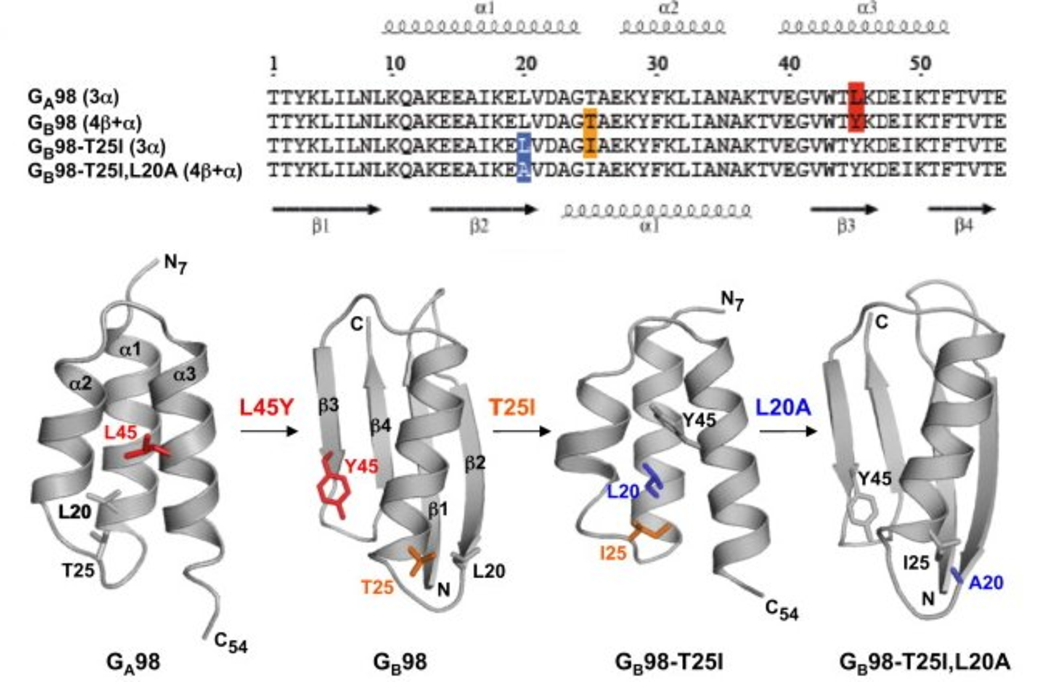
\includegraphics[width=1.0\textwidth]{figures/chameleonic_resume.pdf}
	\caption{Figura da sequencia e das estruturas das camaleonicas}
\end{figure}

\section{Proteínas diversas}

O conjunto de proteínas diversas utilizado para o treinamento do autômato foi obtido do banco de dados “Top8000” ( versão de 2015). Esse banco de dados foi organizado pelo Richardson Lab da Universidade de Duke (disponível em \href{https://github.com/rlabduke/reference_data}{github.com/rlabduke/reference\_data}). As cadeias selecionadas atendem aos seguintes critérios:

\begin{itemize}
	\item{Resolução < 2.0 \AA}
	\item{MolProbity score < 2.0}
	\item{$\le 5 \%$ dos resíduos apresentando comprimentos de ligação anormais ( $> 4\sigma$)}
	\item{$\le 5 \%$ dos resíduos apresentando ângulos de ligação anormais ( $> 4\sigma$)}
	\item{$\le 5 \%$ dos resíduos com desvios anormais do  $C_\beta$ ( > 0.25 \AA)}
\end{itemize}

As cadeias selecionadas pelos critérios acima são subagrupadas de acordo com o grau de identidade sequencial (homologia): < 50\%, <70\% e <95\%.  Cadeias que apresentavam resíduos indeterminados na estrutura ou que apresentaram algum erro durante a atribuição da estrutura secundária por algum dos quatro métodos foram removidos do conjunto. A tabela (?) mostra o número de cadeias utilizadas.

\begin{table}
    \myfloatalign
  \begin{tabularx}{\textwidth}{Xll} \toprule
    \tableheadline{Conjunto}   & \tableheadline{\# original}   & \tableheadline{\# utilizadas}  \\ 
    \midrule
    Top8000-hom50 & 7233 &  6749 \\
    Top8000-hom70 & 7958 & 7435 \\
    Top8000-hom95 & 8826 & 8227 \\
    %autem vulputate ex & parola & romanic \\
    %usu mucius iisque & studio & sanctificatef \\
    \bottomrule
  \end{tabularx}
  \caption[Autem timeam deleniti usu id]{Autem timeam deleniti usu
  id. \citeauthor{knuth:1976}}  \label{tab:example}
\end{table}

